%%%%%%%%%%%%%%%%%%%%%%%%%%%%%%%%%%%%%%%%%
% Hardware AI
% Version 0.1 (09/10/20)
%
% Original author: Logan Fortune
%%%%%%%%%%%%%%%%%%%%%%%%%%%%%%%%%%%%%%%%%%
\documentclass[10pt,letterpaper]{article} 
\usepackage[utf8]{inputenc} 
\usepackage[english]{babel}
\usepackage[T1]{fontenc}
\usepackage[vmargin=1.5cm,hmargin=0.9cm]{geometry}
\usepackage{multicol}
\usepackage{multirow}   
\usepackage{graphicx}   
\usepackage{float} 
\usepackage{listings}
\usepackage{flushend}
\usepackage{minted}
\usepackage[none]{hyphenat} 
\usepackage[small]{caption}
\usepackage{hyperref}
\usepackage{color}      
    \hypersetup{colorlinks=true, linkcolor=[rgb]{0,0,1}, citecolor=[rgb]{0,0,1}}
\usepackage{titlesec}
\usepackage{tikz}
\usetikzlibrary{automata, positioning, arrows}
\tikzset{
    ->,  % makes the edges directed
    node distance=3.5cm, % specifies the minimum distance between two nodes. Change if necessary.
    every state/.style={thick, fill=gray!10}, % sets the properties for each ’state’ node
    initial text=$ $, % sets the text that appears on the start arrow
    }
\renewcommand\thesection{\Roman{section}}
\renewcommand\thesubsection{\Roman{subsection}}
\titlespacing*{\section}{0pt}{2.5mm}{0mm}
\titleformat{\section}[block]{\large\scshape\centering}{\thesection.}{1em}{}
\titleformat{\subsection}[block]{\large}{\thesubsection.}{1em}{}		

%%%%%%%%%%%%%%%%%%%%%%%%%%%%%%%%%%%%%%%%%%%%%%%%%%%%%%%%%%%%%%%%%%%%%%%%%%%%%%

\newcommand{\colorhrule}[3]{\begingroup\color{#1}\rule{#2}{#3}\endgroup}

\setlength{\intextsep}{1mm} 
\setlength{\columnsep}{5mm} 

\begin{document}
\sloppy
\begin{center}
\huge{\textsc{\textbf{Comet Core}}}\\ %\vspace{5mm}
{\footnotesize Logan Fortune, Inria}
\end{center}
	

\begin{center}
\colorhrule{black}{16.5cm}{1.2pt}
\end{center}
\begin{abstract}
\noindent 
% Abstract
\textcolor{red}{This paper should be used for personal use only.} Comet is an open source general purpose central processing unit (CPU) core developed at Inria-Rennes \cite{urlgit}. The architecture is based upon RISCV RV32I base ISA. It is written in $C++$ for High Level Synthesis (HLS). This paper aims to describe with much accuracy this CPU and to present some micro-architectural choices for the multi-core version.
\end{abstract}
\begin{center}
\vspace{-5mm}
\colorhrule{black}{16cm}{0.7pt}
\end{center}

\section{Introduction}\vspace{0.3cm}

Comet is a general purpose processor that is based upon the Harvard architecture as you can see in the figure \ref{fig:macro_one}. It means that the instruction memory and the data one communicate with the core on different buses. Thus, there are two memory interfaces implemented inside the design. The global stall is a signal that forces the core to freeze entirely. It is an external interrupt signal.

\vspace{0.5cm}

\begin{figure}[H]
\centering
\includegraphics[width=7cm]{img/global_macro_1.PNG}
\caption{Comet Macroscopic Overview}
\label{fig:macro_one}
\end{figure}

The architecture core is a five-stage pipeline as you can see in figure \ref{fig:macro_two}: \textit{fetch, decode, execute, memory} and \textit{writeback}. This architecture has a forward and a branch unit making the CPU to run faster but also to stay \underline{consistent} during execution. 

\vspace{0.5cm}

\begin{figure}[H]
\centering
\includegraphics[width=16cm]{img/global_macro_2.PNG}
\caption{Core Architecture Overview}
\label{fig:macro_two}
\end{figure}

This CPU gathers standard design codes and does not have fancy state-of-the-art mechanisms because it mainly targets embedded applications. However, it is still a CPU that is competing in a good position against other RISCV CPUs (like Rocket and PicoRV) in its application range. The code is available at \url{https://gitlab.inria.fr/srokicki/Comet/-/tree/zephyrOS} and will be explained in the next sections.

\section{Pipeline Stages}

\subsection{Fetch}

The fetch stage is designed to monitor the \textit{Program Counter} and the instructions dynamic during execution of the program. It takes the instruction that has been fetched to the instruction memory and send it to the decode stage at the next strike of clock. The main goal is to compute the next program instruction to fetch (see \textit{nextPC\_fetch} in the figure \ref{fig:macro_two}) which is the Program Counter plus four because four bytes is equal to 32 bits and instructions are word-aligned. 

\subsection{Decode}

The decode stage goal is to prepare the instruction to the execution stage. It is strongly based on the RISCV ISA described in the figure \ref{fig:isa} (not including CSR instructions). The decode stage decomposes the instruction into an \textit{opcode} with the type of the operation (\textit{funct7} and \textit{funct3}), \textit{source registers}, a \textit{destination register} and finally an \textit{immediate} value (unless it is a R-type instruction).

\begin{figure}[H]
\centering
\includegraphics[width=12cm]{img/riscv-isa.PNG}
\caption{RISCV ISA Overview}
\label{fig:isa}
\end{figure}

In the decode stage, all possible immediate values (I, S, B, U, J types) are generated. And the correct values are correctly stored inside the \textit{left hand side} (lhs), \textit{right hand side} (rhs) and \textit{datac} registers (see figure \ref{fig:decode}). It is also there that operand values are accessed in the registers file and store in rhs and lhs registers (see figure \ref{fig:decode}). These registers are used by the execution stage right after the forwarding mechanism processing (combinatorial part - multiplexer) to finally compute the operation requested in the execution stage.

\begin{figure}[H]
\centering
\includegraphics[width=8cm]{img/macro_decode.PNG}
\caption{Comet Decode Architecture Overview}
\label{fig:decode}
\end{figure}

There is a special case in the decode stage: the \underline{JAL} opcode. The JAL that stands for \textit{Jump And Link} is an instruction that forces the CPU program counter to jump to the address computed (\textit{nextPC\_decode} in figure \ref{fig:macro_two}) and to store the return address. In this case, the next Program Counter is affected and thus transmitted inside the branch unit with a control signal (\textit{isBranch}) in order to change the program counter of the CPU (\textit{core.pc}) accordingly.

\newpage

\subsection{Execute}

The execution stage computes the operation requested by using lhs, rhs and datac registers according to the combination of the \textit{opcode}, \textit{funct3} and \textit{funct7}. The result of the operation (extoMem.result) or the data (extoMem.datac) to be stored is sent to the memory stage. 

\subsection{Memory}

The memory stage prepares the result to be loaded or stored (RISCV\_LD, RISCV\_ST) inside the data memory thanks to the memory interface. After being processed by the memory stage, the destination register, the value to write and some control signals are sent to the Write Back stage.

\subsection{Write Back}

The write back stage aims to store the result inside the registers file that feeds the decode stage.

\subsection{Branch Unit}

The branch unit aims to deliver a coherent branch execution by taking the different PCs computed inside the Fetch, the Decode or the Execution stage that have been triggered by a branch or a jump instruction. The different modifications of the core execution is represented in the table below. When a branch is taken, it is mandatory to flush some parts of the pipeline in order to keep the execution consistent.

\begin{center}
 \begin{tabular}{||c c c c||} 
 \hline
 Opcode & Branch Resolved in... & Control Signal & Flush Strategy \\ [0.5ex] 
 \hline\hline
 JAL & Decode & isBranch\_decode & Fetch \\ 
 \hline
 BR, JALR & Execute & isBranch\_execute & Fetch and Decode\\
 \hline
\end{tabular}
\end{center}

\subsection{Forward Unit}

The forward unit is a way to get faster execution by moving the execution stage result to the decode operands outputs (only if necessary) instead of waiting the result to be stored in the registers file. In fact, if the execute, the memory or the write back stage will write into a destination register (\textit{executeUseRd}, \textit{memoryUseRd}, \textit{writebackUseRd}) the instruction that will be executed can already use the result to avoid Read After Write (RAW) issue. The forwarding mechanism is just after the decoder stage (see figure \ref{fig:decode}) and modifies the value of the lhs, rhs and datac registers as you can see in figure \ref{fig:fwunit}.

\vspace{0.5cm}

\begin{figure}[H]
\centering
\includegraphics[width=10cm]{img/forward_unit.PNG}
\caption{Comet Forward Unit Overview}
\label{fig:fwunit}
\end{figure}

\newpage

\subsection{Pipeline Stalls}
 
 \subsubsection{Stall Verification Strategy Methodology}
 
 This section aims to elaborate a methodology to check that we get the best strategy for the different signals that stop execution of the core or a sub-section of it. The methodology is the following: \underline{\textit{define all rules}} for all different kind of control signals (global stall, invalidation, etc...) and \underline{\textit{check that all rules}} are accurately applied when a control signal is turned on inside the design. I have developed some global rules in order to optimize as much as possible the stalls used inside the Comet core. It is a personal verification list in order to check that we tend to an optimal strategy. \\
 
\textbf{Definitions:}
 \begin{itemize}
     \item A process inside the core is considered as a sub-system of the core. It can considered as a black-box. It is fully combinatorial or sequential. The granularity of the process precision is chosen as the one provided in the "core.cpp".
     \item A resource is a memory unit that can be used by the processes.
     \item A stall signal is a signal that is used to stop a subset of the core for an undefined amount of time.
     \item An invalidation signal ("*.we" in the cpp code) is a signal that informs the CPU that the targeted instruction should not be considered/processed.
     \item The \textit{isLongInstruction} or \textit{executeIsLongComputation} signals are used to stall the CPU for one cycle to anticipate that a load instruction cannot have its result after the execution stage but after the memory one. This bubble inside the pipeline is mandatory to solve all dependencies issues. 
 \end{itemize}
 
\textbf{Rules:}
 \begin{itemize}
     \item A process can create a stall signal. A stall must not block the process that releases it.
     \item The global stall stops all processes of the design.
     \item A stall must block the propagation of future instructions but not anterior instructions unless they consume the same resource than the process generator of the (un)stall signal.
     \item An invalidation must only invalidate the future instructions that are already in the pipeline. The invalidation signals must be kept along the wrong instructions during their whole propagation inside the pipeline.
 \end{itemize}
 
 The invalidation signal can be used to flush the pipeline in case of an interruption or a taken branch. The stall signal are mainly used to stop a subset of the core during long execution (multiplication, memory communication, flushing procedures).

\subsubsection{Comet Control Signals}
 The core is mainly managed by control signals that ensure no hazards happen due to incorrect timing. That is why the use of \textit{stall signals} are everywhere inside the core. The table below is a synthesis of the influence of all stall signals.
 
\begin{center}
 \begin{tabular}{||c c c c c c c c||} 
 \hline
 Core Process & stallIm* & stallDm & stallFetch** & stallDecode & stallExecute & stallMemory & stallMultAlu \\ [0.5ex] 
 \hline\hline
IM Process &  &  &  &  &  &  &  \\ 
 \hline
DM Process & x &  &  &  &  & x & \\
\hline
Branch unit & x & x & x &  &  &  & x \\
\hline
Forward Unit &  &  &  &  &  &  & \\
\hline
Commit Fetch & x & x & x &  &  &  & x \\
\hline
Commit Decode & x & x &  & x &  &  & x \\
\hline
Commit Execute & x & x &  &  & x &  & x \\
\hline
Commit Memory & x & x &  &  &  & x &  \\
\hline
Regfile Write Back & x & x &  &  &  &  & \\
 \hline
\end{tabular}
\end{center}
* stallIm is a stall for instruction memory interface and stallDm is for the data memory interface.\\
*** stallFetch, stallDecode, etc... is coded in the Comet HLS project as "core.stallSignals[STALL\_FETCH]" and "core.stallSignals[STALL\_DECODE]" respectively for instance.\\
**** A stall signal named \textit{localstall} freezes entirely the pipeline. It does not appear in the table above.\\

The forward unit will not impact the core because the invalidation will make the signal "*.useRd" equal to zero which means that no forwarding is possible.

\begin{figure}[H]
\centering
\includegraphics[width=14cm]{img/invalidation_comet.PNG}
\caption{Comet Invalidation Signals}
\label{fig:cache_invalidation}
\end{figure}

\section{Memory and Cache}

\subsection{Memory Interface}

The memory interface is coded in HLS as a table of $2^{24}$ integers. The address is in 32 bits while there is only $2^{24}$ data. That is why a mask is necessary (0xffffff) to convert the 32 bits address into a 24 bits address. It is interesting to notice that the two least significant bits are avoided because the instructions are word aligned. 

\subsection{Cache Technology}

The Comet cache is a 4-way associative cache. It handles byte (unsigned or not), half (unsigned or not), word or long (maximum limited by the interface size) data size requests (see figure \ref{fig:cache_mask}). The working principle of the cache can be explained with the figures below (figure \ref{fig:cache} and \ref{fig:cache_mask}):

\begin{figure}[H]
\centering
\includegraphics[width=14cm]{img/cache_macro.PNG}
\caption{Comet Cache Architecture Overview}
\label{fig:cache}
\end{figure}

\begin{figure}[H]
\centering
\includegraphics[width=14cm]{img/cache_mask.PNG}
\caption{Comet Cache Possible Access}
\label{fig:cache_mask}
\end{figure}

The cache is the closest level of memory inside the CPU. It is a memory sub-system that is less larger than the external memory. The cache is divided in sets (\textit{set}-associative). And a set is decomposed into four blocks (\textit{four-way} set associative) with each block decomposed also in lines which are byte memory units. Alongside a block of the set, there is a tag which can be compared with the tag address in order to resolve if there is a hit or a miss. There are also registers that store the \textit{age} of the block and a bit that says if the block is a valid memory block. The \textit{age} register is used to update the cache by removing the \textit{least recently used} blocks of the cache. The state machine of the cache can be explained thanks to the figures below (figure \ref{fig:cacheFSM}) . The interesting part of the cache state machine is when there is a miss. When a miss occurs, the most aged cache block of the set must be removed and new values should be inserted instead according to the address requested. The dirty bit of this block is checked because if the dirty bit is equal to zero, it means that the cache block has not been modified since it has been loaded from the main memory. In that case, there is no need to write back the data in the main memory. At contrary, if the dirty bit is equal to one, we need to correct the value in main memory. This mechanism is the origin of the \textit{penalty miss}. While this mechanism could be seen as a burden for the memory interface, it can be proven that caching is efficient thanks to the locality principle which states that \textit{things that will happen soon are likely to be closed to things that just happened}. As you can see in figure \ref{fig:cacheFSM}, this cache has a \textit{write back} policy. It means that the \underline{store} instruction writes effectively only in a cache block without updating the main memory (incoherence may occur) until a \underline{write back} happens from the cache to the main memory.

\begin{figure}[H] 
\centering 
\includegraphics[width=14cm]{img/comet_state_machine.PNG}
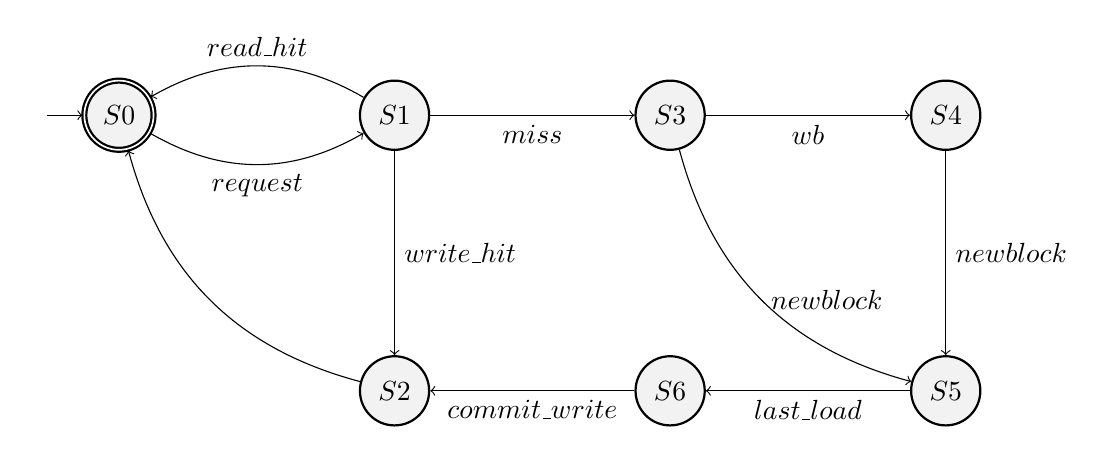
\begin{tikzpicture}
\node[state, initial, accepting] (1) {$S0$};
\node[state, right of=1] (3) {$S1$};
\node[state, below of=3] (2) {$S2$};
\node[state, right of=3] (4) {$S3$};
\node[state, right of=4] (5) {$S4$};
\node[state, below of=5] (6) {$S5$};
\node[state, below of=4] (7) {$S6$};

\draw (1) edge[below, bend right] node{$request$} (3)
(3) edge[above, bend right] node{$read\_hit$} (1)
(3) edge[right] node{$write\_hit$} (2)
(2) edge[below, bend left, right=0.3] node{} (1)
(3) edge[below] node{$miss$} (4)
(4) edge[below] node{$wb$} (5)
(5) edge[right] node{$newblock$} (6)
(6) edge[below] node{$last\_load$} (7)
(4) edge[below, bend right, right=0.3] node{$newblock$} (6)
(7) edge[below] node{$commit\_write$} (2);
\end{tikzpicture}
\caption{Cache Macroscopic Finite State Machine (\textit{wb}: write-back, \textit{newblock}: new cache block)}
\label{fig:cacheFSM}
\end{figure}

The Comet cache can be in different states :

\begin{itemize}
    \item S0: \textit{Neutral} State: the cache is waiting for new instructions.
    \item S1: Cache \textit{request}: the cache is examining to know whether it is a hit or a miss.
    \item S2: Cache \textit{write}: the cache writes into one of its sub-block (see figure \ref{fig:cache}).
    \item S3: The cache enters in the \textit{miss} sub-states: the cache chooses the right cache block to evict. Then it sends the first memory request to elaborate a \textit{the write-back} (Store) or to acquire the first chunk of the new cache block (Load).
    \item S4: In the this state the cache is doing write-backs (see figure \ref{fig:cacheFSM}).
    \item S5: In the this state the cache acquires cache blocks (see figure \ref{fig:cacheFSM}).
    \item S6: The cache leaves the \textit{miss} sub-states, the cache is ready to write the new cache block. In this state, we do not yet write to the cache and we do not send a memory request. We just acquires the last memory chunk. 
\end{itemize}

\newpage

\section{Operating System Specific Architecture}\vspace{0.3cm}

An operating system (OS) is a software that is used to ease the management between user applications and hardware. Especially, the operating system schedules tasks and guarantees safe execution of the programs. We decided that \textbf{ZephyrOS} (\textit{Linux Foundation}) will be the first OS to be booted with Comet. ZephyrOS is an operating system for embedded systems. This OS is close to Linux which can allow a smooth transition toward it. ZephyrOS is open-source with long-term support (LTS) with security updates.

\subsection{Control State Registers (CSR)}

The control state registers is used to gather statistics about the working core (like the number of instructions retired \textit{minstret}, the counters \textit{mhpmcounter3} or simply the number of cycles \textit{mcycle}). It is also where the current core status is stored (inside \textit{mstatus}). There are finally specific CSRs that are central in the making of exceptions and interruptions management. 

\subsection{Core-Local Interrupt Controller (CLINT)}

The core-local interrupt controller is an element outside the core. We can access this element by making a memory call (memory-map). The goal of this block is to give a precise timer (\textit{mtime}) independent of the execution of the program. It is also a way to prepare an interruption at a specific moment written inside the \textit{mtimecmp} register.

\subsection{Exceptions and Interruptions}

Exceptions and interruptions are special triggers that change the normal execution of the program. An exception is raised by the program to elaborate a specific routine like a thread switch or a break (debug). The interruption is created outside the core (e.g CLINT). It changes the program execution the same way as the interruption but the handler of those calls will know if this is an interruption or an exception (see \textit{mcause}). When returning from an exception or an interruption, we need to continue the program left thanks to a special register that store the previous program counter (\textit{mepc}).

\subsection{Memory Map}

In order to boot ZephyrOS with the core, the OS should have a memory map of all elements of the board described in the \textit{device tree}. This memory map is the image of the environment allowing the core to communicate efficiently with all modules (see figure \ref{fig:memoryMap} - this figure is subject to change).

\begin{figure}[H]
\begin{center}
 \begin{tabular}{||c c c c||} 
 \hline
 Base & Length & Attributes & Description \\ [0.5ex] 
 \hline\hline
 0x0000\_0010 & 0x0000\_0300 &  & CLINT \\ 
 \hline
 0x0000\_0310 & 0x0000\_0480 & & (Early Console) Secure Enclave \\
\hline
 0x0000\_0790 & 0x0000\_07A8 & & UART (LiteUART from LiteX) \\
\hline
 0x0003\_0000 & ND & EX, NI, C & ROM + DRAM \\
\hline
\end{tabular}
\end{center}
\caption{Memory Map (EX: Executable, NI: Non-idempotent, C: Cached, ND: Not defined)}
\label{fig:memoryMap}
\end{figure}

\subsection{Uart - Console}

The UART is a serial communication that aims to communicate information to external modules (included humans one). We used the UART to simulate a screen. There is also an early console that can be used to check the boot sequence. Indeed, the early console is a special zone in memory that aims to store specific data during boot sequence as you can see in figure \ref{fig:zephyrboot_img}. This part of the memory can also be used during execution for very specific purposes (security strategy, external data feed, etc...).\\

\begin{figure}[H]
\centering
\includegraphics[width=16cm]{img/hello_world_comet_zephyr.png}
\caption{Zephyr Boot Sequence Demo}
\label{fig:zephyrboot_img}
\end{figure}

\section{Testing Procedures And Benchmark}\vspace{0.3cm}

Comet core is coded in C++ which allows an easier way to describe the hardware. With the work done in Inria-Rennes \cite{paper}, the HDL generated by the HLS tool should be equivalent to the C++ simulation. Thus, the designer should only be worried about the high level description of the core and all tests can be done with the C++ emulation. This workflow is a great opportunity for the CPU designer to evaluate quickly a micro-architecture but also to test it more easily by gathering the strengths of the C++ language and the community that comes with it. The workflow developed in Inria tries to be at best compliant with the RISC-V community last requirements. 

\begin{figure}[H]
\centering
\includegraphics[width=15cm]{img/comet_workflow.PNG}
\caption{Comet Core Workflow}
\label{fig:comet_workflow}
\end{figure}

\subsection{Compliance Suite}

The compliance suite is a series of unitary tests that aims to evaluate if the hardware design is \textit{RISC-V compliant} according to the ISA specification. RISC-V is an open-source standard ISA with lots of freedom given to the architects. That is why it is important to always ensure to pass the conformance testing preventing from fragmentation of the hardware developments (\url{https://semiengineering.com/toward-risc-v-compliance/}). These tests used all the instructions of the ISA. The tool feeds the core with specific instructions and checks each time the output signature.

\subsection{Hand-Written Test}

Hand-written tests are tests created at the beginning of the creation of comet. There are four tests that cover algorithms like djikstra, sorting methods, etc... These tests are more complex than the unitary ones. The reference model used to check the validity of the tests is the cpu of your computer.

\subsection{Embench}

In order to get an overview of the core performance, we added a benchmark named Embench. This benchmark targets embedded central processing units. It is a way to compare ourselves with other central processing units (\url{https://antmicro.github.io/embench-tester/}) but also to verify if any new implementation of Comet has not impacted the performance overall.

\subsection{M-CVM}

M-CVM is a tool created especially to test comet with a multi-core configuration. This is a way to ensure that the multi-core system can work efficiently and without major deadlocks. Multi-core systems are an ensemble of central processing units. They can together execute unrelated programs or they share the same working data.  When cores share their memories, there needs extra hardware to allow consistent memory communications and to force coherency between cores.The coherency protocol is hard to verify as the cardinal of the tests space skyrockets with the number of cores. Moreover, it is still difficult to find some bare-metal RISC-V tests for multi-core systems. Indeed, most of the time, the tests provided consider that the system can boot an operating system (see litmus tests).

\newpage

\section{Core HLS}

\subsection{HLS in a nutshell}

HLS stands for \textit{High Level Synthesis}. The idea is to get a higher level of abstraction of hardware design. The C++ language is used to describe the architecture. And Catapult HLS tool chain transforms this description into a netlist format in vhdl (or verilog) that can be used inside your favorite FPGA or ASIC tool chains. Even if the level of abstraction is high, the hardware designer must still think about how the design elaborated in C++ could be synthesized in hardware. However, the burden of architecture optimization and simplification is entirely managed by the HLS tool.

\subsection{Comet-Catapult workflow}

This section aims to describe how the core is used by the Catapult HLS tool. The result of the HLS tool is a VHDL or Verilog netlist of the design. The HLS flow can be described as follow:

\begin{figure}[H]
\centering
\includegraphics[width=14cm]{img/hls_flow.PNG}
\caption{HLS Synthesis Flow}
\label{fig:HLS_synth}
\end{figure}

The HLS flow imposed by Catapult begins by giving the C++ design and useful scripts in order to synthesize correctly the design. The firsts step is the hierarchy organization description. During this step, the aim is to define what is the top design and the related hierarchical blocks. Just after that, we link the different hardware units with a production technology (ST Microelectronics, Intel, etc...). Then, one of the most important step is the architecture phase which defines memories types and memories organization. The memory type is the technology (RAM, ROM, etc...) while the memory organization is about data placement inside the memory. Finally, Catapult will elaborate the rtl design (vhdl/verilog output file - concat\_rtl.vhdl) according to the previous constraints.

\begin{figure}[H]
\centering
\includegraphics[width=14cm]{img/HLS_flow.png}
\caption{Catapult Flow}
\label{fig:catapult}
\end{figure}

\newpage

\section{Multi-Core Comet}

\subsection{Introduction to multi-core}

The making of a multi-core architecture is a challenge that must involve both software and hardware coherency. The following section will separate the multi-core challenge in three parts: software, ISA and hardware architecture. The software part will focus on parallelism limits and the different challenges underlying such a programming strategy. The ISA part is the frontier between the software and the hardware design. We will see what kind of extensions must be provided to the Comet core in order to obtain a complete multi-core system. Then, the hardware part will focus mainly on the memory system and especially the caches. 

\subsection{Multi-processing Software}

\subsubsection{Multi-core applications}

Multi-processing software is undeniably an efficient way to obtain faster results provided that we can set up parallel calculations. For instance, an embedded system that makes cryptography computations and at the same time does independently machine learning prediction would appreciate to have a dual core processor to compute faster these two threads. However, if the program is a tightly sequential algorithm, the burden created by separating the processing between two cores may not justify the cost (silicon, energy, computation time). There is not a linear progression between the speedup and the amount of processors you can use in parallel \underline{for a fixed problem size}. Indeed, the gain in speedup follows the well-known \underline{Amdahl} law. There is another law, the Gustafon's law, claiming that in practice we set the size of the problems to fully exploit the computing power so that we have a different performance prediction. The Gustafon'law "is based on the approximations that the parallel part scales linearly with the amount of resources, and that the serial part does not increase with respect to the size of the problem" \cite{url1}.

\begin{itemize}
    \item \textbf{Amdahl} : $speedup = \frac{1}{s+\frac{p}{N}}$
    \item \textbf{Gustafon}: $scaled\_speedup = s + p * N$
\end{itemize}

where s is the proportion of execution time spent on the serial part, p is the proportion of execution time spent on the part that can be parallelized, and N is the number of processors.

\begin{figure}[H]
\centering
\includegraphics[width=10cm]{img/multi_proc/Amdahl_laws.png}
\includegraphics[width=10cm]{img/multi_proc/gustafon_laws.PNG}
\caption{Amdahl's Law}
\label{fig:amdahl}
\end{figure}

\subsubsection{Multi-processing Challenges}

\textbf{The first challenge} to solve when considering multi-processing program is how the memory is seen by the programmer. Indeed, the hardware can provide two types of memories for multi-core architecture: \textit{shared memory} or \textit{distributed memory}. The two different memory architectures imply two different ways to program:\\
\begin{itemize}
    \item \textit{With the shared memory}, data and instructions are seen by all the cores without restrictions. The programmer does not have to think about the distribution of the data (or the instructions) among the cores.
    \item \textit{With the distributed memory}, the programmer needs to explicitly determine how the data and the instructions memory should be split among the cores. This method allows a core to work independently without interfering too much with other cores. If a core needs to communicate with another one, there is a special protocol named "\textit{Message Passing}" that transfer the shared data.
\end{itemize}

The advantages and drawbacks of the two strategies can be resumed with the following table:

\begin{center}
 \begin{tabular}{||c c c||} 
 \hline
  & Message Passing & Shared Memory \\ [0.5ex] 
 \hline\hline
 Communication & Programmer & Automatic \\ 
 \hline
 Data Distribution & Manual & Automatic \\
\hline
 Hardware Support & Simple & Extensive \\
\hline
 Programming & Explicit - Specific compiler & \\
\hline
 Correctness & difficult & less difficult \\
\hline
 Performance & difficult & very difficult \\
\hline
\end{tabular}
\end{center}

\vspace{0.3cm}

The message passing strategy forces the programmer to think with much details how each core acts on the data. This kind of strategy imposes that the programmer will by himself do the data distribution among the cores. At contrary, the shared memory model will automatically do the distribution but the programmer has to carefully add some synchronization code snippets in order to have a coherent execution of the program. We will use the \textit{shared memory} strategy because of the ease of programming for the core user. Moreover, there is lower overhead (latency) and a better use of bandwidth when communicating small items between cores. There is also less remote communications thanks to the automatic caching of the data.\\

\textbf{The second challenge} that comes with the shared memory strategy is the \textit{synchronization}. To understand synchronization, an example is necessary. The following example uses two threads for counting occurrences of letters of a string. The first thread counts the first half of the string while the second one counts the second half.

\begin{verbatim}
    Core 0                 |      Core 1
   1. LW L, 0(R1) # L="A"         LW L, 0(R1) # L="A"  
   2. LW R, Count[L] # 15         LW R, Count[L] # 15
   3. ADD R, R, 1 # 16            ADD R, R, 1 # 16
   4. SW R, Count[L] # 16         SW R, Count[L] # 16
\end{verbatim}

In this example, because the two threads can simultaneously without synchronization between them, instead of counting A two times, it will maybe count A only once (line 3 is done the same time). In order to have a correct program execution, it needs to protect the critical section (between lines 2 and 4) with a lock (see the solution below): it is called \textit{synchronization}.

\begin{verbatim}
    Core 0                 |      Core 1
   1. LW L, 0(R1) # L="A"         LW L, 0(R1) # L="A"  
   LOCK                           LOCK
   2. LW R, Count[L] # 15         LW R, Count[L] # 15
   3. ADD R, R, 1 # 16            ADD R, R, 1 # 16
   4. SW R, Count[L] # 16         SW R, Count[L] # 16
   UNLOCK                         UNLOCK
\end{verbatim}

The lock mechanism authorizes only one core to enter inside the part between the lock and the unlock. The lock can be implemented thanks to a simple variable and atomic instructions (see RISCV ISA part). This synchronization issue is fundamental to multi-processing programming. There is another type of synchronization called "\textit{barrier synchronization}". The barrier is often used when a program needs to wait the results of multiple threads before going forward. The idea is that all threads must arrive to the barrier before any can leave it. A lot of programming challenges can be deduced with this simple example but they are mainly caused by the \textit{memory consistency}.\\

\textbf{The third challenge} is the memory consistency model. While coherency defines order of accesses to the same address, consistency defines order accesses to different addresses. We need a memory model in order to define the rules. The model is the contract between the software and the implementation about the set of legal behaviors. A simple answer to what is a memory consistency model is that it specifies the values that can be returned by loads \cite{url2}. Again, an example will help to explain this challenge:

\begin{verbatim}
        Core 0   |  Core 1
        A = 0       B = 0
        A = 1       B = 1
    L1: if(B==0)    if(A==0)
\end{verbatim}

The condition L1 can easily give the following answers (False, False), (True, False) or (False, True). But suppose the write invalidate is delayed, and the processor is allowed to continue during this delay; then it is possible that both Core 0 and Core 1 have not seen the invalidation for B and A (respectively) before they attempt to read the values. The question is, should this behavior be allowed, and if so, under what conditions ? The most straightforward model for memory consistency is called \textit{sequential consistency}. Sequential consistency requires that the result of any execution be the same as if the accesses executed by each processor were kept in order and the accesses among different processors were interleaved. Sequential consistency ensures that all memory accesses execute as if we process them one at a time, each time selecting a core and letting it complete its next access in program order. Note that this does not require round-robin selection of cores – it even allows one core to be selected several times in a row. This allows for many possible interleaving of accesses from different cores, but it prevents accesses from one core from being reordered. But this consistency model is very bad for performance. That is why there are some \underline{relaxed models} that give better performances but at the expense of a less predictable program execution.

For instance, consider the following situation:

\begin{verbatim}
    Thread 0:               Thread 1:
    D=1;                printf("L:%d ", L);
    L=1;                printf("D:%d ", D);
\end{verbatim}

Under \textit{sequential consistency}, the possible outputs are L:0 D:0 (if Thread 0 does both of its accesses after Thread 1 prints both variables), L:1 D:1 (if Thread 0 does both accesses before Thread 1 prints them), or L:0 D:1 (if Thread 1 prints L, then Thread 1 modifies D, and then thread 1 prints D). The outcome of L:1 D:0 cannot happen because the printout of L:1 means that Thread 0 did its L=1 access, and sequential consistency ensues that by that time D=1 is also complete so D:0 cannot be printed after printing L:1. In contrast, \textit{weak consistency} allows the two accesses in Thread 0 to be reordered, in which case it is possible to print out L:1 D:0 (print both L and D in Thread 1 after L=1 has executed but before D=1 is executed in thread 0). The different consistency model can be resumed with the following graphs (see figure \ref{fig:consistency_model}):

\begin{figure}[H]
\centering
\includegraphics[width=15cm]{img/multi_proc/consistency_models.PNG}
\caption{Consistency Models \cite{book}}
\label{fig:consistency_model}
\end{figure}

In order to solve issues that result from consistency models (like data races for instance), synchronization methods can help but there are also special instructions called FENCE that force ordering of instructions by saying that no other core can observe any operation (instructions) in the successor set following a FENCE before any operation in the predecessor set preceding the FENCE.

\subsection{RISCV ISA}

\subsubsection{RISCV Memory Model (RVWMO) - Atomic Operations}

The memory model of RISCV is named the RVWMO model. RVWMO stands for RISC-V Weak Memory Ordering. This memory model is defined thanks to axioms. A RISC-V hardware implementation is allowed as long as it does not fail to respect any axioms (see figure \ref{fig:rvwmo} in Annexes). The Comet core supports the 32-bits base Integer RISCV ISA. In order to have a multi-core system, the ISA must be extended to have atomic operations (A) and Zicsr extensions.

Atomic operations are mandatory to create a multi-core system. These operations prevent a core to modify a specific variable while another core has decided otherwise. There are three important atomic operations: \textit{Load-Reserve, Store-Conditional, Swap-Write}. More atomic operations are possible but they can be re-created at a low-level software layer with only the three atomic operations aforesaid. 

The \textit{Load-Reserve} instruction is a basic load at a memory address given by the user. This load is special because it will save the address at a specific register named the \textit{registration register} and will validate a bit (named \textit{aq} bit here) that is associated with this register. The \textit{Load-Reserve} instructions is always associated with the \textit{Store-Conditional} to build lock-free data structures. "An SC instruction can never be observed by another RISC-V hart before the LR instruction that established the reservation." (RISC-V ISA specification) The \textit{Store-Conditional} is a write that is effectively done \textit{if and only if} the registration register is equal to the address of the store and if the \textit{aq} bit is high. If a core X has written to the address saved in the registration register of the core Y before the Store-Conditional and after the Load-Reserve of the core Y, the \textit{aq} bit of the core Y will be invalidated. Regardless of success or failure, executing a Store-Conditional instruction invalidates any reservation held by this hart. If the Store-Conditional is successful, the core will be notified by receiving an answer from the cache: a zero. At contrary, if unsuccessful, it will receive a one. The \textit{Swap-Write} reads the data at the memory address specified as if it was a load and writes after, at the same address, a new value given by the instruction as if it was a store.

\begin{figure}[H]
\centering
\includegraphics[width=14cm]{img/multi_proc/atomic_op.PNG}
\caption{Atomic Operations}
\label{fig:atomicop}
\end{figure}

\subsection{Multi-core Architecture}

The benefits of having multi-core hardware system should not be seen as obvious as we saw with the Amdahl's law. It is sometimes more interesting to have a better single core with less silicon area, better energy consumption and better \textit{instruction per cycle} (IPC). But it can be proven that there are diminishing returns to optimize too much a single core. Moreover, one solution to get a better core is to increase the frequency and thus the voltage which is directly linked to the power (cubic relation). Thus a dual-core can have better benefits than a single very optimized processor (and vice versa).\\

Let us do a simple example to convince ourselves that this is not as simple. If we have a single core processor that takes 1$cm^2$ silicon area with an IPC equal to 2.5 working at 50W for 2GHz, there are two strategies possible to improve the hardware system: a better single core or more cores. With the first strategy, we can obtain, for example, a new core with an IPC of 3.5 taking 2 $cm^2$ silicon area at 75W for 2.2 GHz. The second strategy can get a multi-core system taking obviously 2$cm^2$ with single cores that work with an IPC of 2.5. They totally spent 100W at 2 GHz. The speedup of the first strategy is 1.1 (frequency optimization) * 1.4 (IPC optimization) = 1.5 while the second one is 2 \textit{assuming that the program can simply be divided among cores}. 

\newpage

\subsubsection{Global Strategy}

The first thing that must be think when considering multi-core hardware system is how to ensure memory coherence and especially cache coherence. Indeed, each core has its own cache which implies a coherency issue that can be illustrated with the following problem:

\begin{verbatim}
    A = 0
    
    Core 0     |  Core 1
    .             .
    Lw R0 <= A    .
    R0++          .
    Sw R0 => A    .
    .             .
    .             Lw R0 <= A
    .             R0++
    .             Sw R0 => A
\end{verbatim}

We need to ensure that Core 1 will write 2 to A. This can be done if Core 0 informs to Core 1 the new value of A which is stored in its cache. This is called \textit{cache coherency}. There are \textbf{three requirements} to get cache coherency:

\begin{itemize}
    \item A Read address X on core 0 returns the value written by the most recent write to X on core 0 if no other core has written to X in between.
    \item  If core 0 writes to X and core 1 reads after a sufficient time, and there are no other writes in between, core 1's read returns the value from core 0's write.
    \item Writes to the same location are serialized: any two writes to X must be seen to occur in the same order on all cores.
\end{itemize}

There are two steps for creating a hardware implementation with cache coherency. First, you need to decide how to broadcast information about cache blocks modifications: you can either broadcast writes in a shared bus (\textit{snooping protocol}) or use a central directory (\textit{directory-based}). Then, you need to choose how you update data in all caches: you can either update all values (\textit{write-update}) or invalidate blocks that are no longer valid (\textit{write-invalidate}). The differences between the write-update and the write-invalidate protocol can be resumed in the table below:

\begin{center}
 \begin{tabular}{||c c c||} 
 \hline
 Application does... & Update & Invalidate \\ [0.5ex] 
 \hline\hline
 Burst of writes to one address & Each write sends an update (Bad) & First write invalidates (Good)\\ 
 \hline
 Write different words in the same block & Each write sends an update (Bad) & First write invalidates (Good)\\
\hline
 Producer/consumer & Updates to consumers (Best) & Prod Inv Cons misses (Bad)\\
\hline
\end{tabular}
\end{center}

It appears that write-invalidate is slightly stronger, especially when there is an OS that transfer a thread to another core because the write-update could keep updating the old thread related to the old core's cache.

\subsubsection{Multi-core Cache Controller - MSI Protocol}

The global multi-core architecture chosen is a write-invalidate protocol with a directory based shared memory. This strategy can be resumed with the following figure \ref{fig:mem_dir}:\\

\begin{figure}[H]
\centering
\includegraphics[width=12cm]{img/multi_proc/multi_core_mem.PNG}
\caption{Memory Architecture}
\label{fig:mem_dir}
\end{figure}

\newpage

\noindent We have created a specific protocol that aims to communicate efficiently with the directory (see figure \ref{fig:mem_dir}). The main challenge for the cache L1 is to be able to send an instruction to the cache L2 but also to be able to answer to specific requests sent by the cache L2.

\begin{verbatim}

/* Basic Interface Skeleton */
struct cacheDirectoryInterfaceBase {
  // in or out
  ac_int<32, false> addr;
  ac_int<1, false> interfaceAck;
  ac_int<1, false> releaseAck;
};

/* Buffer Out / WB Interface */
typedef struct cacheDirectoryInterfaceOut : public cacheDirectoryInterfaceBase {
  memOpType interfaceRequest;
  // data out
  ac_int<32, false> buffer;
  // data In
  ac_int<32, false> bufferIn;
} cacheDirectoryInterfaceOut;

/* Buffer In Interface */
typedef struct cacheDirectoryInterfaceIn : public cacheDirectoryInterfaceBase {
  ac_int<1, false> protocolMiss;
  directoryOpType interfaceRequest;
} cacheDirectoryInterfaceIn;

/* Cache L2 Interface --> Out */
typedef struct cacheL2DirectoryInterfaceOut : public cacheDirectoryInterfaceBase {
  // data out
  ac_int<32, false> buffer;
  ac_int<1, false> protocolMiss;
  directoryOpType  interfaceRequest;
  ac_int<4, false> hartid;
  ac_int<1, false> cache;
} cacheL2DirectoryInterfaceOut;

/* Cache L2 Interface --> In */
typedef struct cacheL2DirectoryInterfaceIn : public cacheDirectoryInterfaceBase {
  // in to cache
  memOpType interfaceRequest;
  ac_int<4, false> hartid;
  ac_int<1, false> cache;
  // out from cache 
  ac_int<32, false> dataLoad;
  ac_int<1, false> protocolMiss;
  ac_int<1, false> rejection;
  // Special WB input
  ac_int<1, false> interfaceAckWB;
  ac_int<1, false> releaseAckWB;
  ac_int<32, false> addrWB;
  // data in
  ac_int<32, false> buffer;
  ac_int<32, false> bufferWB;
} cacheL2DirectoryInterfaceIn;



typedef struct directoryStruct {

  cacheStatus cacheStateDir = INVALID;             // cache status
  ac_int<log2const<NB_CORES>::value, false> owner; // Who is the owner ?
  ac_int<NB_CORES, false> sharers   = 0;           // Which cores are sharing the data ?
  ac_int<NB_CORES, false> coreToken = 0;           // Does a core use this directory line ?

} directoryStruct;
\end{verbatim}

This protocol provides a way to manage caches dynamic by sending information to the directory or to the caches. There are two different types of request: directory requests and cache requests.

\begin{center}
\begin{tabular}{ |p{6cm}||p{6cm}|  }
 \hline
 Requests & Goal\\
 \hline
 \multicolumn{2}{|c|}{Directory} \\
 \hline
 REQ\_INV   & Request for invalidation of a cache block \\
 \hline
 REQ\_DATATRANSFER\_INV&  Request to send a cache block and invalidate it after \\
 \hline
 REQ\_DATATRANSFER\_SHARED & Request to send a cache block and change cache status to SHARED \\
 \hline
 \multicolumn{2}{|c|}{Cache} \\
 \hline
 LOAD &   Load a data at a specific address.\\
 \hline
 STORE & Store a data at a specific address.\\
 \hline
 WRITEBACK & Send a cache line to the next level of caches.\\
 \hline
 WRITEHIT & Send a cache write hit. Other caches sharing this cache block must be invalidated.\\
 \hline
 AMO\_(LR/SC/SWAPW) &  Atomic operations requests. \\
 \hline
 MISS\_(WRITE/READ) & Ask for permission to enter in a miss state.\\
 \hline
 END\_MISS & Request to release the cache lock inside the directory.\\
 \hline
\end{tabular}
\end{center}

\noindent The cache keeps its previous FSM but we have now added a specific sub-FSM (orange and blue links in figure \ref{fig:cachemultiFSM}) for atomic operations and directory requests. The C++ design of the cache tries to be at much as possible close a single core cache FSM in order to limit the silicon surface by re-using existing sub-FSM. 

\begin{figure}[H] 
\centering 
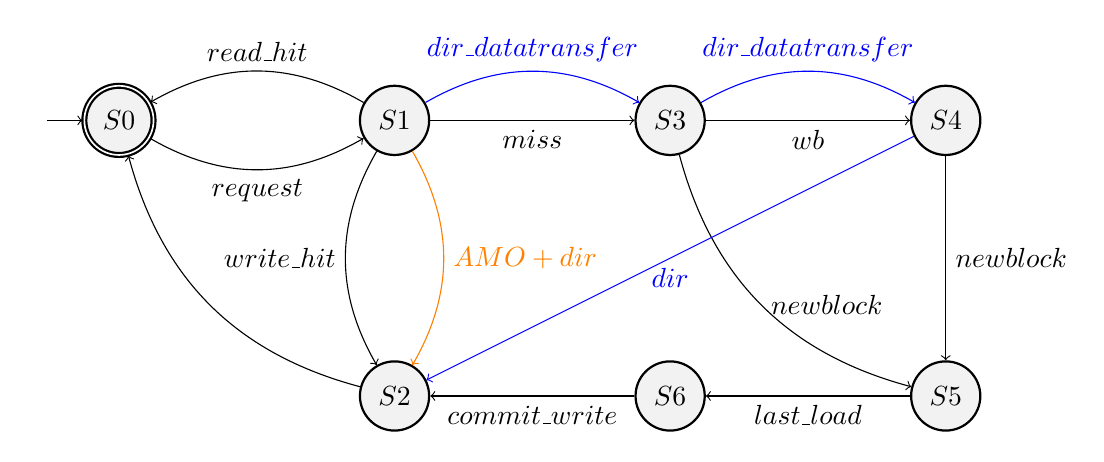
\begin{tikzpicture}
\node[state, initial, accepting] (1) {$S0$};
\node[state, right of=1] (3) {$S1$};
\node[state, below of=3] (2) {$S2$};
\node[state, right of=3] (4) {$S3$};
\node[state, right of=4] (5) {$S4$};
\node[state, below of=5] (6) {$S5$};
\node[state, below of=4] (7) {$S6$};

\draw (1) edge[below, bend right] node{$request$} (3)
(3) edge[above, bend right] node{$read\_hit$} (1)
(3) edge[left, bend right, left=0.3] node{$write\_hit$} (2)
(3) edge[below, bend left, right=0.3, orange] node{$AMO + dir$} (2)
(2) edge[below, bend left, right=0.3] node{} (1)
(3) edge[below] node{$miss$} (4)
(4) edge[below] node{$wb$} (5)
(5) edge[right] node{$newblock$} (6)
(6) edge[below] node{$last\_load$} (7)
(4) edge[below, bend right, right=0.3] node{$newblock$} (6)
(7) edge[below] node{$commit\_write$} (2)
(3) edge[above, bend left, blue] node{$dir\_datatransfer$} (4)
(4) edge[above, bend left, blue] node{$dir\_datatransfer$} (5)
(5) edge[below = 0.5, blue] node{$dir$} (2);
\end{tikzpicture}
\caption{Cache Macroscopic \textit{Incomplete} Finite State Machine (\textit{wb}: write-back, \textit{newblock}: new cache block, \textit{dir}: directory request, \textit{AMO}: atomic operations) for a multi-core system.}
\label{fig:cachemultiFSM}
\end{figure}

\noindent But this FSM is incomplete because there are multiple strategies possible that prioritize instructions from the directory given by the cache controller and the core given by the current instruction inside the core:

\begin{itemize}
    \item Directory requests over core instructions.
    \item Core instructions over the directory requests.
    \item First in, first taken.
\end{itemize}

\noindent The only viable strategy is that directory requests are prioritized over core instructions. Indeed, if we let the cores instructions be prioritized, there will be possible deadlocks when processors need each other at the same time. The directory is the chief of the operations and should cleverly allocate priorities precisely to each core at the right moment as we will see in the next part.\\

\noindent The previous FSM must be augmented in order to get some in-between states that ensure the cache can go forward without creating some incoherence between the cores. In order to get an efficient multi-core design, we also must avoid to overwhelm the directory with requests. Indeed, a request to the directory costs at least one cycle of penalty. For instance, if we have a write hit, the cache with the hit must warn the others but not always as you can see in the table below:\\

\begin{table}[H]
\begin{center}
\begin{tabular}{||c c c c ||} 
 \hline
 Cache Status & Next Cache Status & Directory Need (Y/N) & Penalties \\ [0.5ex] 
 \hline\hline
 Exclusive & Modified & Y (change directory state) & 1 cycle \\
 \hline
 Shared & Modified & Y (REQ\_INV) & $\geq 3$ cycles \\
 \hline
 Modified & Modified & N & 0 cycle\\
 \hline
\end{tabular}
\caption{Cache Status Dynamic - Write Hit}
\label{fig:cacheStatusDyn_hitwrite}
\end{center}
\end{table}

\begin{table}[H]
\begin{center}
\begin{tabular}{||c c ||} 
 \hline
 Cache Status & Write-Back (Y/N) \\ [0.5ex] 
 \hline\hline
 Invalid & N\\
 \hline
 Exclusive & N\\
 \hline
 Shared & N\\
 \hline
 Modified & Y (4 cycles penalties)\\
 \hline
\end{tabular}
\caption{Cache Status Dynamic - Write Back}
\label{fig:cacheStatusDyn_writeback}
\end{center}
\end{table}

The miss state is a special state of the cache. During a miss state, the cache will not receive a directory request (guarantee by the directory). This state will block the others cache that would like to use that specific cache for any reasons (Write Hit, Miss Write, Miss Read, etc.). 

\begin{figure}[H] 
\centering 
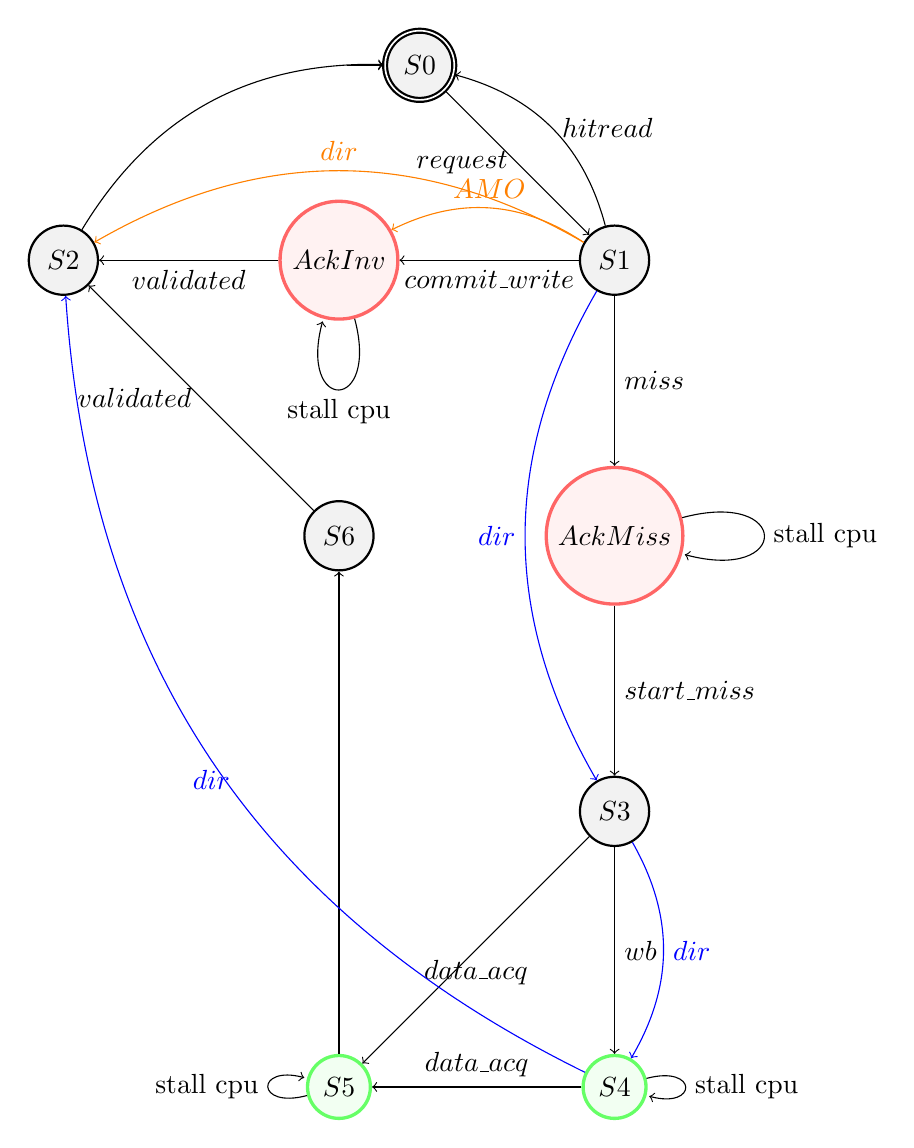
\begin{tikzpicture}[roundnode/.style={circle, draw=green!60, fill=green!5, very thick, minimum size=5mm}, roundnodespec/.style={circle, draw=red!60, fill=red!5, very thick, minimum size=5mm}]
\node[state, initial, accepting] (1) {$S0$};
\node[state, below right of=1] (3) {$S1$};
\node[roundnodespec, left of=3] (8) {$AckInv$};
\node[state, left of=8] (2) {$S2$};
\node[state, below of=8] (7) {$S6$};
\node[roundnodespec, below of=3] (11) {$AckMiss$};
\node[state, below of=11] (4) {$S3$};
\node[roundnode, below of=4] (9) {$S4$};
\node[roundnode, left of=9] (10) {$S5$};

\draw (1) edge[left] node{$request$} (3)
(3) edge[above, bend right, right=0.3] node{$hitread$} (1)
(3) edge[above, bend right, orange] node{$AMO$} (8)
(3) edge[above, bend right, orange] node{$dir$} (2)
(3) edge[below] node{$commit\_write$} (8)
(2) edge[below, bend left, right=0.3] node{} (1)
(4) edge[below] node{$data\_acq$} (10)
(7) edge[left] node{$validated$} (2)
(8) edge[below] node{$validated$} (2)
(4) edge[right] node{$wb$} (9)
(10) edge[right] node{} (7)
(9) edge[above] node{$data\_acq$} (10)
(9) edge[loop right] node{stall cpu} (9)
(8) edge[loop below] node{stall cpu} (8)
(3) edge[right] node{$miss$} (11)
(11) edge[right] node{$start\_miss$} (4)
(11) edge[loop right] node{stall cpu} (11)
(10) edge[loop left] node{stall cpu} (10)
(3) edge[above=0.3, bend right, left= 0.3, blue] node{$dir$} (4)
(4) edge[above, bend left, right=0.3, blue] node{$dir$} (9)
(9) edge[below = 0.5, bend left, blue] node{$dir$} (2);
\end{tikzpicture}
\caption{Cache Controller CacheToDirectory (1/2) Macroscopic FSM}
\label{fig:cacheCFSM}
\end{figure}

\begin{itemize}
    \item S0: There is no need to communicate something.
     \item S1: 
     \begin{itemize}
         \item [Read Hit:] Do nothing.
         \item [Write Hit:] It must send a request to the directory to invalidate "sharers" (when in a Shared/Exclusive cache state).
         \item [Miss:] It must send a request to the directory for a miss encountered at the specific address.
     \end{itemize}
    \item S2: 
    \begin{itemize}
        \item [Hit Write:] I must write only if all other "\textit{sharers}" have been invalidated (AckInv).
        \item [Miss:] I must commit changes for the new cache block.
        \item [Directory:] I must change the cache status of the cache block selected.
    \end{itemize}
    It must always correctly set the cache status (Exclusive vs Shared vs Modified vs Invalidate).
    \item S3/S4: We perform the write-back (WB) or data fetching if the directory has granted us (AckMiss).
    \item S5: We should get the data needed for the new cache block.
    \item S6: We end the communication with the directory.
\end{itemize}

\begin{figure}[H]
\centering
\includegraphics[width=12cm]{img/multi_proc/hit_wave.png}
\caption{Write Hit Protocol Multi-core}
\label{fig:wh_multicore}
\end{figure}

\begin{figure}[H]
\centering
\includegraphics[width=15cm]{img/multi_proc/multicore_miss_write.png}
\caption{Write Miss Protocol Multi-core}
\label{fig:wm_multicore}
\end{figure}

\noindent We are going to enumerate all the possible necessary communications from a directory request to a cache. Directory requests have higher priorities to core requests. When a request is seen by the cache, all current procedures is halted. It is thus mandatory to be able to get back to the right execution after the directory request is done. There are three types of requests:

\begin{itemize}
    \item Invalidation
    \item Data transfer with invalidation
    \item Data transfer with shared or owner status
\end{itemize}

\noindent During a directory request, the cache controller can be in different states:

\begin{itemize}
    \item D0: no request.
    \item D1: seeking the cache block to modify.
    \item D2: modification of the cache block status (Invalid/Shared).
    \item D3: Send data to the directory for another cache using mechanism of the write-back.
\end{itemize}

\begin{figure}[H] 
\centering 
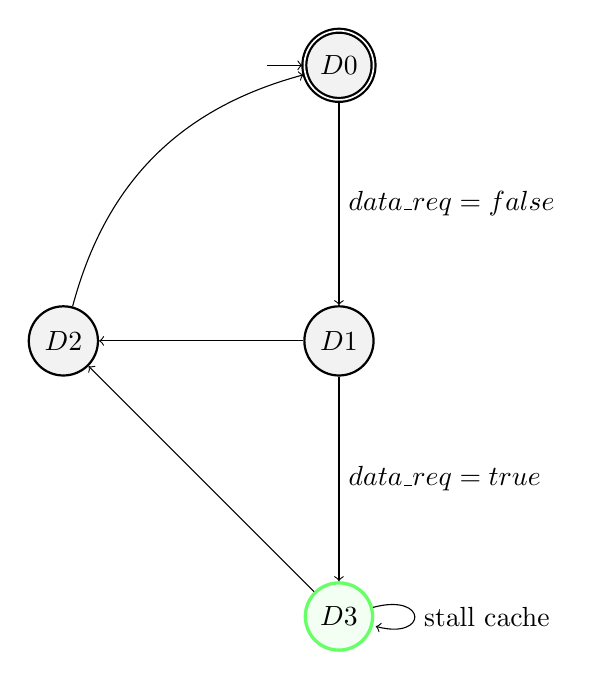
\begin{tikzpicture}[roundnode/.style={circle, draw=green!60, fill=green!5, very thick, minimum size=5mm}]
\node[state, initial, accepting] (1) {$D0$};
\node[state, below of=1] (2) {$D1$};
\node[state, left of=2] (3) {$D2$};
\node[roundnode, below of=2] (4) {$D3$};

\draw (1) edge[right] node{$data\_req = false$} (2)
(2) edge[below] node{} (3)
(3) edge[above, bend left, right=0.3] node{} (1)
(2) edge[right] node{$data\_req = true$} (4)
(4) edge[below] node{} (3)
(4) edge[loop right] node{stall cache} (4);

\end{tikzpicture}
\caption{Cache Controller DirectoryToCache (2/2) Macroscopic FSM}
\label{fig:cacheC2FSM}
\end{figure}

\section{Annexes}

\begin{figure}[H]
\centering
\includegraphics[width=12cm]{img/multi_proc/rvwmo_riscv.PNG}
\includegraphics[width=12cm]{img/multi_proc/rvwmo_rules_riscv.PNG}
\caption{RVWMO - NVIDIA Slide \cite{url2}}
\label{fig:rvwmo}
\end{figure}

\begin{thebibliography}{1} 

\bibitem{urlgit} Comet CPU RISCV HLS
\newblock{\url{https://gitlab.inria.fr/srokicki/Comet}}.
\newblock Inria-Rennes, Simon Ronkicki

\bibitem{paper} Simon Rokicki, Davide Pala, Joseph Paturel, Olivier Sentieys.
\newblock{\textit{What You Simulate Is What You Synthesize: Design of a RISC-V Core from C++ Specifications.}}
\newblock RISC-V Workshop 2019, Jun 2019,Zurich, Switzerland. pp.1-2.

\bibitem{url1} Xin Li
\newblock{\textit{Scalability: strong and weak scaling}}
\newblock \url{https://www.kth.se/blogs/pdc/2018/11/scalability-strong-and-weak-scaling/}, KTH blog.

\bibitem{book} David A. Patterson, John L. Hennessy
\newblock{\textit{Computer Organization and Design - The Hardware/Software Interface}}
\newblock Morgan Kaufmann Publishers

\bibitem{url2} Dan Lustig
\newblock{\textit{Memory Model}}
\newblock \url{https://www.youtube.com/watch?v=QkbWgCSAEoo}, RISCV

\end{thebibliography}

\end{document}